\documentclass{beamer}
\usepackage{myslide2019}
\usepackage[hangul]{kotex}  % Uncomment when if you want Korean writing

\title{Example of Beamer Template Slide }
\subtitle{Subtitle is here}
\author[my name in footer]{My Name In title}
\institute[OrganizationI/Section]
{
  %\inst{1}%
  Your Institute \\
  department \\
  section}
%  \and
%  \inst{2}%
%  Anther \\
%  anther }
\date{\today}
\logo{
\includegraphics[scale=0.3]{Figures/yourlogo.png}} % Put your logo here!
\includeonly{Seminar-DPD-Reference}

% User defined background color for beamerboxesrounded
\xdefinecolor{myTitle0} {cmyk}{0.6,0,1,0}
\xdefinecolor{myTitle1} {cmyk}{0,0,0.6,0.6}
\xdefinecolor{myTitle2} {cmyk}{0.8,0.6,0,0}
\xdefinecolor{myTitle3} {cmyk}{0.6,0.6,0,0}
\xdefinecolor{myTitle4} {cmyk}{0,0.6,0.8,0}
\xdefinecolor{myTitle5} {cmyk}{0,0,0.4,0.4}
\xdefinecolor{myTitle6} {cmyk}{0.6,0.4,1,0}
\xdefinecolor{mySubTitle} {cmyk}{0,0,0.2,0}

\begin{document}

% Title Page is here!
\frame{\titlepage}
%\frame{\tableofcontents}

% First Slide

%%%%%%%%%%%%%%%%%%%%%%%%%%%%%%%%%%%%%%%%%%%%%%%%%%%%%%%%%%%%%%%%%%%%%%%%%%%%%%%%%%%%%%%%%
% New Slide is here!
%%%%%%%%%%%%%%%%%%%%%%%%%%%%%%%%%%%%%%%%%%%%%%%%%%%%%%%%%%%%%%%%%%%%%%%%%%%%%%%%%%%%%%%%%
\begin{frame}
\frametitle{Beamerboxersrounded}

  \setbeamercolor{uppercol}{fg=white,bg=myTitle1}%
  \setbeamercolor{lowercol}{fg=black,bg=mySubTitle}%
  \begin{beamerboxesrounded}[upper=uppercol,lower=lowercol,shadow=true]
  {비선형성에 의한 영향}
  증폭기의 비선형성으로 고조파(Harmonic) 성분과, 혼변조(Intermodulation) 발생함.   사용대역의 신호을 왜곡하고 옆 대역의 신호에 간섭을 주게 됨.
  \begin{itemize}
    \item {\bf Harmonic: } 원래 입력된 신호원천주파수(Fundamental Frequency)의 정수배 주파수 성분이 발생하는 현상
    \item {\bf Intermodulation: } 혼변조(Intermodulation)이란 비선형 소자를 통한 RF 신호처리 과정에서, 두 개의 다른 입력 주파수 신호의
  fundamental 및 harmonic 주파수들 끼리의 합과 차로 조합된 출력 주파수 성분이 나오는 현상

  \end{itemize}
 \end{beamerboxesrounded}
\end{frame}



%%%%%%%%%%%%%%%%%%%%%%%%%%%%%%%%%%%%%%%%%%%%%%%%%%%%%%%%%%%%%%%%%%%%%%%%%%%%%%%%%%%%%%%%%
% New Slide is here!
%%%%%%%%%%%%%%%%%%%%%%%%%%%%%%%%%%%%%%%%%%%%%%%%%%%%%%%%%%%%%%%%%%%%%%%%%%%%%%%%%%%%%%%%%
\begin{frame}
\frametitle{Include figure}

\begin{figure}[h]
\begin{center}
   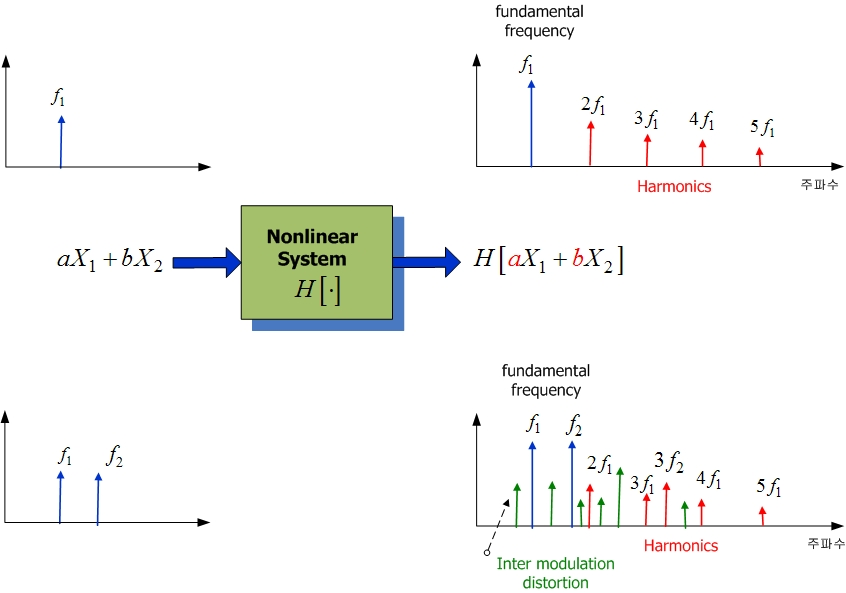
\includegraphics[scale=0.3]{Figures/Nonlinear.jpg}
   \caption{Nonlinear system의 입출력 관계}
  \label{fig:nonlinear}
\end{center}
\end{figure}
\end{frame}

%%%%%%%%%%%%%%%%%%%%%%%%%%%%%%%%%%%%%%%%%%%%%%%%%%%%%%%%%%%%%%%%%%%%%%%%%%%%%%%%%%%%%%%%%
% New Slide is here!
%%%%%%%%%%%%%%%%%%%%%%%%%%%%%%%%%%%%%%%%%%%%%%%%%%%%%%%%%%%%%%%%%%%%%%%%%%%%%%%%%%%%%%%%%
\begin{frame}[shrink=50]
% Styles as before
\frametitle{Include tikz figure}

\begin{figure}
\begin{center}
\begin{tikzpicture}
  \path[mindmap,concept color=black,text=white]
    node[concept] {Computer Science}
    [clockwise from=0]
    child[concept color=green!50!black] {
      node[concept] {practical}
      [clockwise from=90]
      child { node[concept] {algorithms} }
      child { node[concept] {data structures} }
      child { node[concept] {pro\-gramming languages} }
      child { node[concept] {software engineer\-ing} }
    }
    child[concept color=blue] {
      node[concept] {applied}
      [clockwise from=-30]
      child { node[concept] {databases} }
      child { node[concept] {WWW} }
    }
    child[concept color=red] { node[concept] {technical} }
    child[concept color=orange] { node[concept] {theoretical} };
\end{tikzpicture}
\end{center}

\end{figure}


\end{frame}

%%%%%%%%%%%%%%%%%%%%%%%%%%%%%%%%%%%%%%%%%%%%%%%%%%%%%%%%%%%%%%%%%%%%%%%%%%%%%%%%%%%%%%%%%
% New Slide is here!
%%%%%%%%%%%%%%%%%%%%%%%%%%%%%%%%%%%%%%%%%%%%%%%%%%%%%%%%%%%%%%%%%%%%%%%%%%%%%%%%%%%%%%%%%
\begin{frame}
% Styles as before
\frametitle{Include tikz figure 2}

% FSK modulation example figure
\begin{figure}[htp]
\centering

\begin{tikzpicture}[scale=0.4]
 %\documentclass{standalone}
%\usepackage{tikz}
%\usetikzlibrary{shapes}
%\usepackage{pgfplots}

\newcommand{\drawfsk}[4] {
  \draw [smooth,samples=200,#1,domain=#2:#3] plot (\x, {cos(#4*\x r)}); 
  %\draw [smooth,samples=200,#1,domain=#2:#3] plot (\x, {cos(#4*2*pi*\x r)}); 
}


%\begin{tikzpicture}[scale=1]
% Draw FSK signal
\drawfsk{red}{0}{2*pi}{8}
\drawfsk{blue}{2*pi}{4*pi}{4}
\drawfsk{red}{4*pi}{6*pi}{8}
\drawfsk{blue}{6*pi}{8*pi}{4}

\node at (pi,1.5) {$f_1$};
\node at (3*pi,1.5) {$f_2$};
\node at (5*pi,1.5) {$f_1$};
\node at (7*pi,1.5) {$f_2$};

\draw[dashed] (2*pi,-1.5) -- (2*pi,6);
\draw[dashed] (4*pi,-1.5) -- (4*pi,6);
\draw[dashed] (6*pi,-1.5) -- (6*pi,6);
\draw[dashed] (8*pi,-1.5) -- (8*pi,6);

\draw[<->] (0,1.5) node[above] {$s(t)$}  -- (0,0)
   -- (8*pi+1,0) node[right] {$t$};
\draw[->] (0,0) -- (0,-1.5);

\begin{scope}[yshift=3cm]

\draw[<->] (0,2.5) node[above] {$m(t)$}  -- (0,0)
   -- (8*pi+1,0) node[right] {$t$};

% Draw message pulse
\draw [red,ultra thick] (0,0) -- (0,1) -- (2*pi,1) -- (2*pi,0) --
    (4*pi,0) -- (4*pi,1) -- (6*pi,1) -- (6*pi,0) --
	(8*pi,0);

\draw [|<->|,black,dashed] (0,1.5) -- (2*pi,1.5);
\node at (pi,2) {$T_s$};

\end{scope}

%\end{tikzpicture}
%\end{document}
\end{tikzpicture}

\caption{Binary FSK 파형의 예}
\label{fig:fsk}
\end{figure}


\end{frame}

%%%%%%%%%%%%%%%%%%%%%%%%%%%%%%%%%%%%%%%%%%%%%%%%%%%%%%%%%%%%%%%%%%%%%%%%%%%%%%%%%%%%%%%%%
% New Slide is here!
%%%%%%%%%%%%%%%%%%%%%%%%%%%%%%%%%%%%%%%%%%%%%%%%%%%%%%%%%%%%%%%%%%%%%%%%%%%%%%%%%%%%%%%%%
\begin{frame}
\frametitle{Equation}

% FSK passband model 
\begin{equation} \label{eq:ble-fsk}
  s(t) = \left\{
     \begin{array}{lr}
       s_1(t) = A \cos(2 \pi f_c + 2 \pi f_d t) & \text{for binary 1, } 0 \leq t \leq T_s \\
       s_2(t)= A \cos(2 \pi f_c - 2 \pi f_d t) & \text{for binary 0, } 0 \leq t \leq T_s 
    \end{array} \right.  % No space between \end{array} and \right.
\end{equation}

\end{frame}

%%%%%%%%%%%%%%%%%%%%%%%%%%%%%%%%%%%%%%%%%%%%%%%%%%%%%%%%%%%%%%%%%%%%%%%%%%%%%%%%%%%%%%%%%
% New Slide is here!
%%%%%%%%%%%%%%%%%%%%%%%%%%%%%%%%%%%%%%%%%%%%%%%%%%%%%%%%%%%%%%%%%%%%%%%%%%%%%%%%%%%%%%%%%
\begin{frame}
\frametitle{Enumerate}

\begin{figure}[h]
\centering  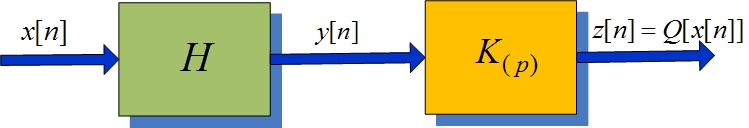
\includegraphics[width=3in]{Figures/volterra.jpg}
\end{figure}


  \begin{enumerate}
    \item 비선형 시스템이 volterra로 표현될 때, p차 volterra inverse 시스템의 post inverse와 pre inverse는 같다.
  \item 비선형 시스템의 $H_1$(선형 부문)의 역함수가 causal이고 stable이면 p차 volterra inverse는 causal이고 stable하다.
   \item pth order inverse filter를 구하는 방법은 일단 pth order volterra $H$를 구한 다음(RLS, LMS등을 사용할 수도 있음),
   $H$와 inverse와의 volterra kernel 관계식을 이용해서 inverse filter를 구한다.

  \end{enumerate}

\end{frame}


%%%%%%%%%%%%%%%%%%%%%%%%%%%%%%%%%%%%%%%%%%%%%%%%%%%%%%%%%%%%%%%%%%%%%%%%%%%%%%%%%%%%%%%%%
% New Slide is here!
%%%%%%%%%%%%%%%%%%%%%%%%%%%%%%%%%%%%%%%%%%%%%%%%%%%%%%%%%%%%%%%%%%%%%%%%%%%%%%%%%%%%%%%%%
% References Slide
\begin{frame}
\frametitle{Rerences}

\begin{thebibliography}{10}
\tiny

\bibitem{RFDH:internet}
``{RF 기초강의실: 선형성정복}.''
\url{http://www.rfdh.com/}.

\bibitem{Rako:internet}
P.~Rako, ``{Heads and tails: Design RF amplifiers for linearity and
  efficiency},'' 2008.

  \url{http://www.ednasia.com/article-20948-headsandtailsdesignrfamplifiersfor%
linearityandefficiency-Asia.html}.

\bibitem{BLE:book2010}
변계섭, 임성화, 이병훈, and 윤종욱, {\em 블루투스 저에너지
  무선기술}. 홍릉과학출판사, 2010.

\bibitem{Psaltis:1988}
D.~Psaltis, A.~Sideris, and A.~A. Yamamura, ``{A multilayered neural network
  controller},'' {\em IEEE Contr. Syst. Mag.}, pp.~17--21, April 1988.

\bibitem{EunCS:1997}
C.~Eun and E.~J. Powers, ``{A New Volterra Predistorter Based on the Indirect
  Learning Architecture},'' {\em IEEE Trans. Signal Processing}, vol.~45,
  pp.~223--227, Jan. 1997.

\bibitem{LimSM:2006}
임선민, 은창수, ``{p차 역필터 기법을 이용한 OFDM
  시스템의 메모리가 없는 비선형 고전력 증폭기의 전치
  보상기 설계},'' {\em 한국통신학회논문지}, vol.~31,
  pp.~191--199, Feb. 2006.

\bibitem{LimSM:internet}
임선민, 은창수, ``{간접 학습 구조를 이용한 비선형
  고전력 증폭기의 전치 보상기의 설계},
 \url{http://mnet.skku.ac.kr/data/2003data/KICS2003/pdf/15-61.pdf}, 2003.

\bibitem{Liu2017}
J.~Liu and M.~Cai, ``{GFSK} modulation for {BLE} baseband {IC} design,'' in
  {\em 2017 International Conference on Electron Devices and Solid-State
  Circuits ({EDSSC})}, {IEEE}, oct 2017.

\bibitem{Saleh:1981}
A.~A.~M. Saleh, ``{Frequency-independent and frequency-dependent nonlinear
  models of TWT amplifiers},'' {\em {IEEE} Trans. Commun.}, vol.~29,
  pp.~1715--1720, Nov. 1981.


\end{thebibliography}  

\end{frame}

\end{document}

